\documentclass{beamer}

\usepackage{graphicx}
\usepackage{mathtools}
\usepackage{mathrsfs}
\usepackage{fdsymbol}
\usepackage{hyperref}

%Information to be included in the title page:
\title{Multivariate Causal Models}
\author{Congyuan Duan}
%\institute{School of Mathematics, Sun Yat-sen University}



\begin{document}

\frame{\titlepage}

\begin{frame}
    \frametitle{Contents}
    \tableofcontents
\end{frame}

\section{Calculating Intervention Distributions by Covariate Adjustment}

\begin{frame}
    \frametitle{Contents}
    \tableofcontents[currentsection]
\end{frame}

\begin{frame}
    \frametitle{Calculating intervention distributions}
    \begin{flushleft}
        Problem: the intervention distribution is unknown, and we do not have data from it.  
    \end{flushleft} 
    \centering{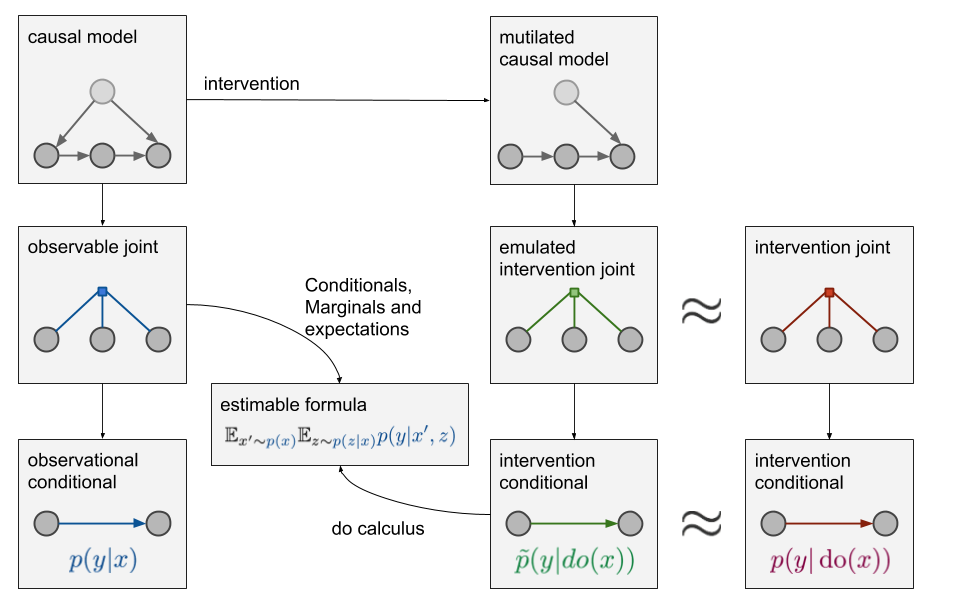
\includegraphics[scale=0.3]{fig4.png}}
\end{frame}

\begin{frame}
    \frametitle{Independence assumption}
    \begin{flushleft}
        If we intervene on a variable, then the other mechanisms remain invariant.  Given an SCM $\mathfrak{C}$, and 
        intervening on $X_k$ but not on $X_j$, we have
    \end{flushleft} 
    \begin{align*}
        p^{\widetilde{\mathfrak{C}}}(x_j|x_{pa(j)})=p^{\mathfrak{C}}(x_j|x_{pa(j)})
    \end{align*}
    \begin{flushleft}
        This allows us to compute statements about intervention distributions even though we have never seen data from it.
    \end{flushleft}
\end{frame}

\begin{frame}
    \frametitle{Truncated factorization}
    \centering{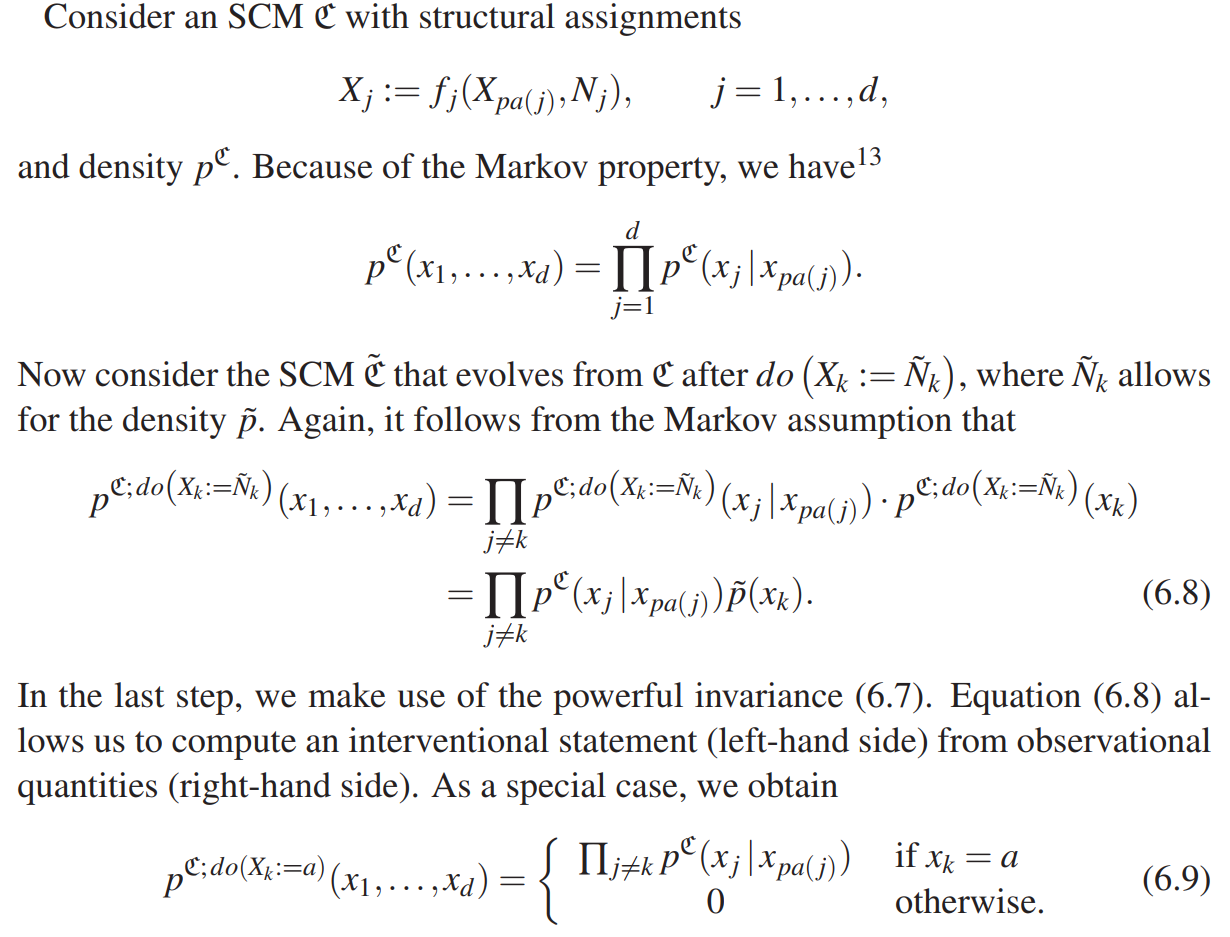
\includegraphics[scale=0.6]{fig5.png}}
\end{frame}

\begin{frame}
    \frametitle{Special case}
    \begin{flushleft}
        Conditioning and intervening are different operations, but they become identical for variables that do not have 
        any parents.
    \end{flushleft}
    \centering{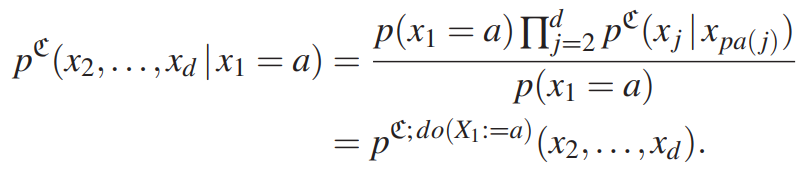
\includegraphics[scale=0.6]{fig6.png}}
\end{frame}

\begin{frame}
    \frametitle{Example: Kidney stones, continued}
    \centering{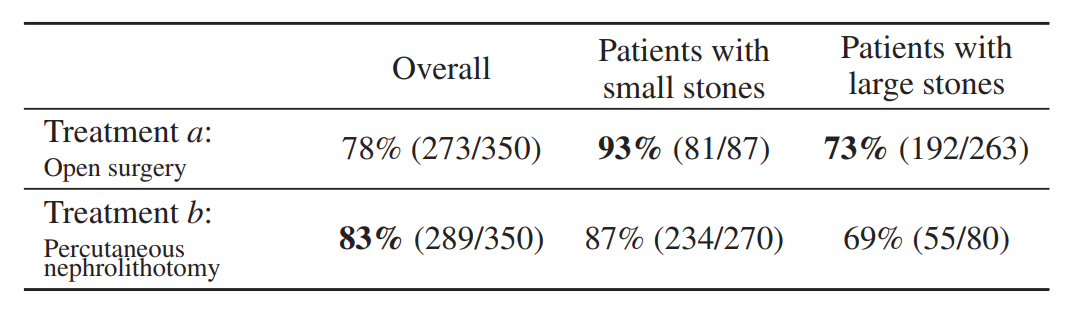
\includegraphics[scale=0.6]{fig7.png}}
    \centering{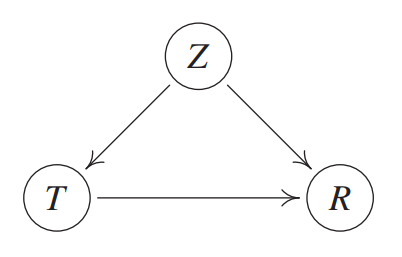
\includegraphics[scale=0.6]{fig8.png}}
    \centering{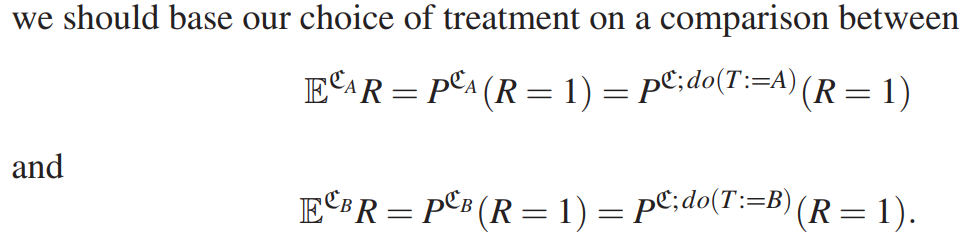
\includegraphics[scale=0.6]{fig9.png}}
\end{frame}

\begin{frame}
    \frametitle{Example: Kidney stones, continued}
    \centering{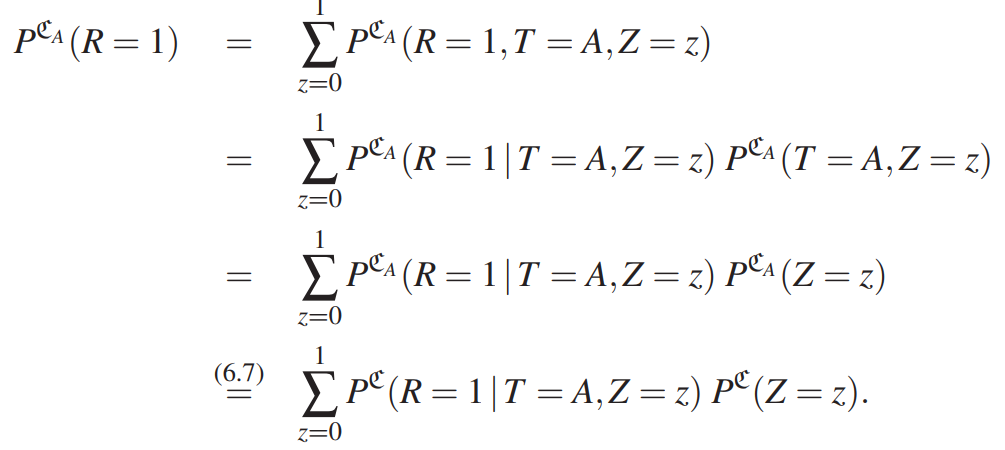
\includegraphics[scale=0.6]{fig10.png}}
    \begin{flushleft}
        The last equation is called "adjusting" for the variable $Z$.
    \end{flushleft}
\end{frame}

\begin{frame}
    \frametitle{Example: Kidney stones, continued}
    \centering{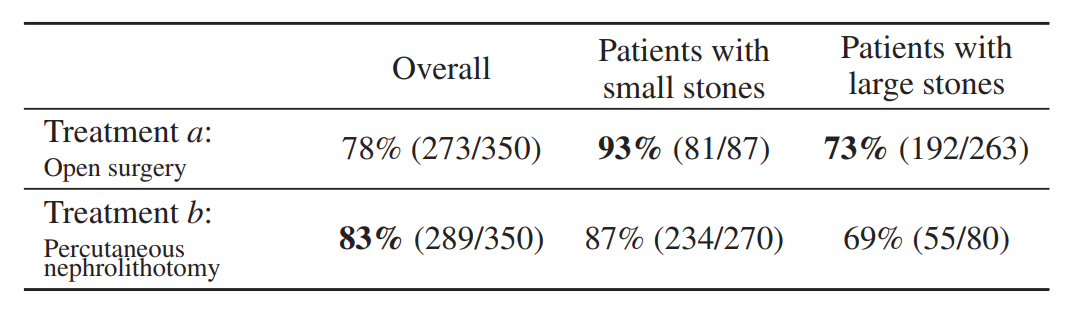
\includegraphics[scale=0.6]{fig7.png}}
    \leftline{With the data in the table}
    \centering{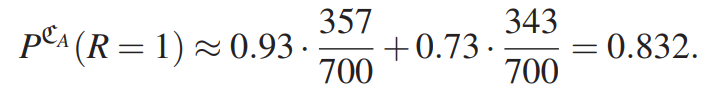
\includegraphics[scale=0.6]{fig26.png}}
    \centering{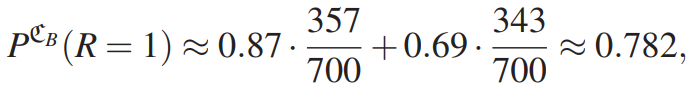
\includegraphics[scale=0.6]{fig27.png}}
    \begin{flushleft}
        This example also shows the difference between conditioning and intervention.
    \end{flushleft}
    \centering{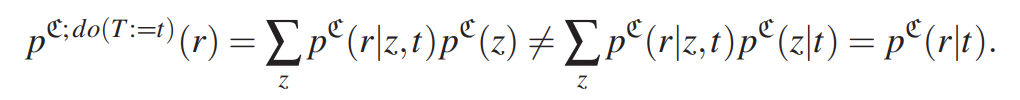
\includegraphics[scale=0.6]{fig11.png}}
    \centering{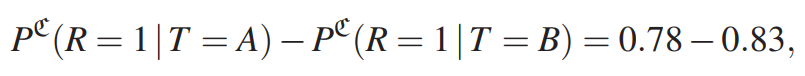
\includegraphics[scale=0.6]{fig28.png}}
\end{frame}

\begin{frame}
    \frametitle{Valid adjustment set and confounding}
    \centering{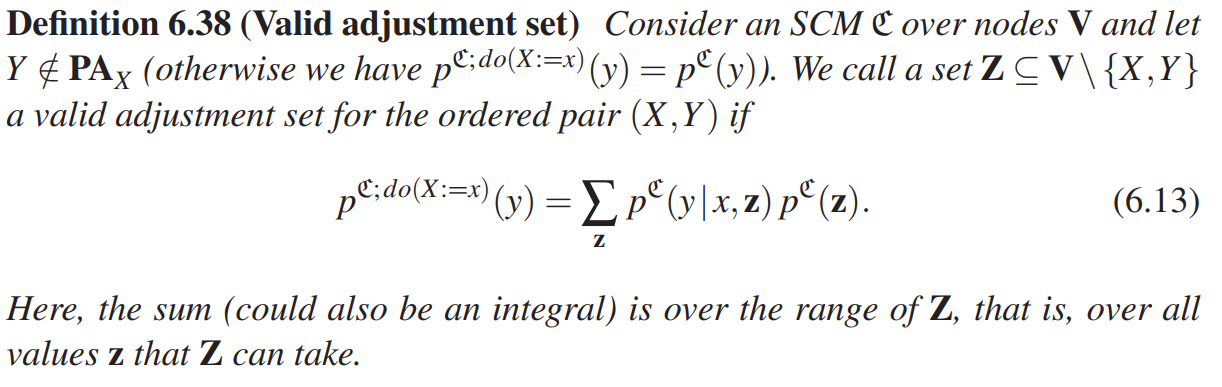
\includegraphics[scale=0.6]{fig12.png}}
    \begin{flushleft}
        When the empty set is not a valid adjustment set, we say that the causal effect is confounded.
    \end{flushleft}
    \centering{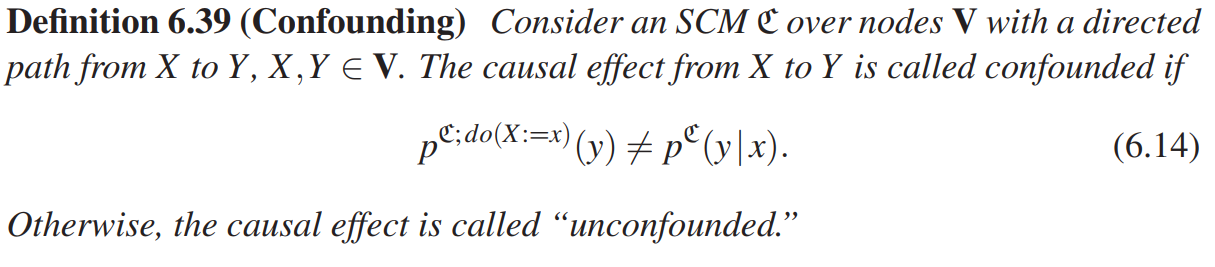
\includegraphics[scale=0.6]{fig13.png}}
\end{frame}

\begin{frame}
    \frametitle{Valid adjustment set and confounding}
    In the last example, for any set $Z$,
    \begin{align*}
        p^{\mathfrak{C};do(X:=x)}(y) &= \sum_z p^{\mathfrak{C};do(X:=x)}(y,z) \\
        &= \sum_z p^{\mathfrak{C};do(X:=x)}(y|x,z)p^{\mathfrak{C};do(X:=x)}(z)
    \end{align*}
    If we have
    \begin{align*}
        &p^{\mathfrak{C};do(X:=x)}(y|x,z) = p^{\mathfrak{C}}(y|x,z) \\
        &p^{\mathfrak{C};do(X:=x)}(z) = p^{\mathfrak{C}}(z)
    \end{align*}
    \begin{flushleft}
        it follows that $Z$ is a valid adjustment set. We thus need to address the question of which conditionals remain
        invariant under the intervention $do(X:=x)$.
    \end{flushleft}
\end{frame}

\begin{frame}
    \frametitle{Characterization of invariant conditionals}
    \begin{flushleft}
        We construct a new SCM $\mathfrak{C}^*$ that equals $\mathfrak{C}$ but has one more variable $I$ that indicates whether 
        the intervention took place or not. $I$ is a parent of $X_k$ and does not have any other neighbors. 
    \end{flushleft}
    \centering{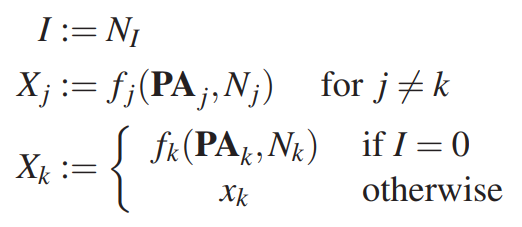
\includegraphics[scale=0.6]{fig14.png}}
    \begin{flushleft}
        $I=0$ corresponds to the observational setting and $I=1$ to the interventional setting. We have
    \end{flushleft}
    \begin{align*}
        p^{\mathfrak{C}^*}(x_1,\cdots,x_d|I=0) &= p^{\mathfrak{C}^*;do(I:=0)}(x_1,\cdots,x_d) \\
        &= p^{\mathfrak{C}^*}(x_1,\cdots,x_d)
    \end{align*}
    \leftline{and}
    \begin{align*}
        p^{\mathfrak{C}^*}(x_1,\cdots,x_d|I=1) &= p^{\mathfrak{C}^*;do(X_k:=x_k)}(x_1,\cdots,x_d)
    \end{align*}
\end{frame}

\begin{frame}
    \frametitle{Characterization of invariant conditionals}
    \begin{flushleft}
        Using the Markov condition for $\mathfrak{C}^*$, it thus follows for variables $A$ and a set of
        variables $B$ that
    \end{flushleft}
    \centering{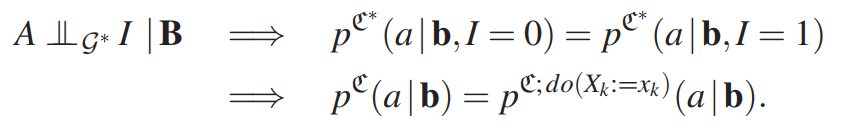
\includegraphics[scale=0.6]{fig15.png}}
    \leftline{So we need to find $Z$ such that}
    \centering{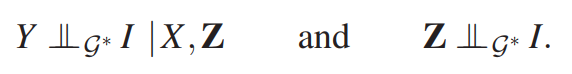
\includegraphics[scale=0.6]{fig16.png}}
\end{frame}

\begin{frame}
    \frametitle{Valid adjustment sets}
    \centering{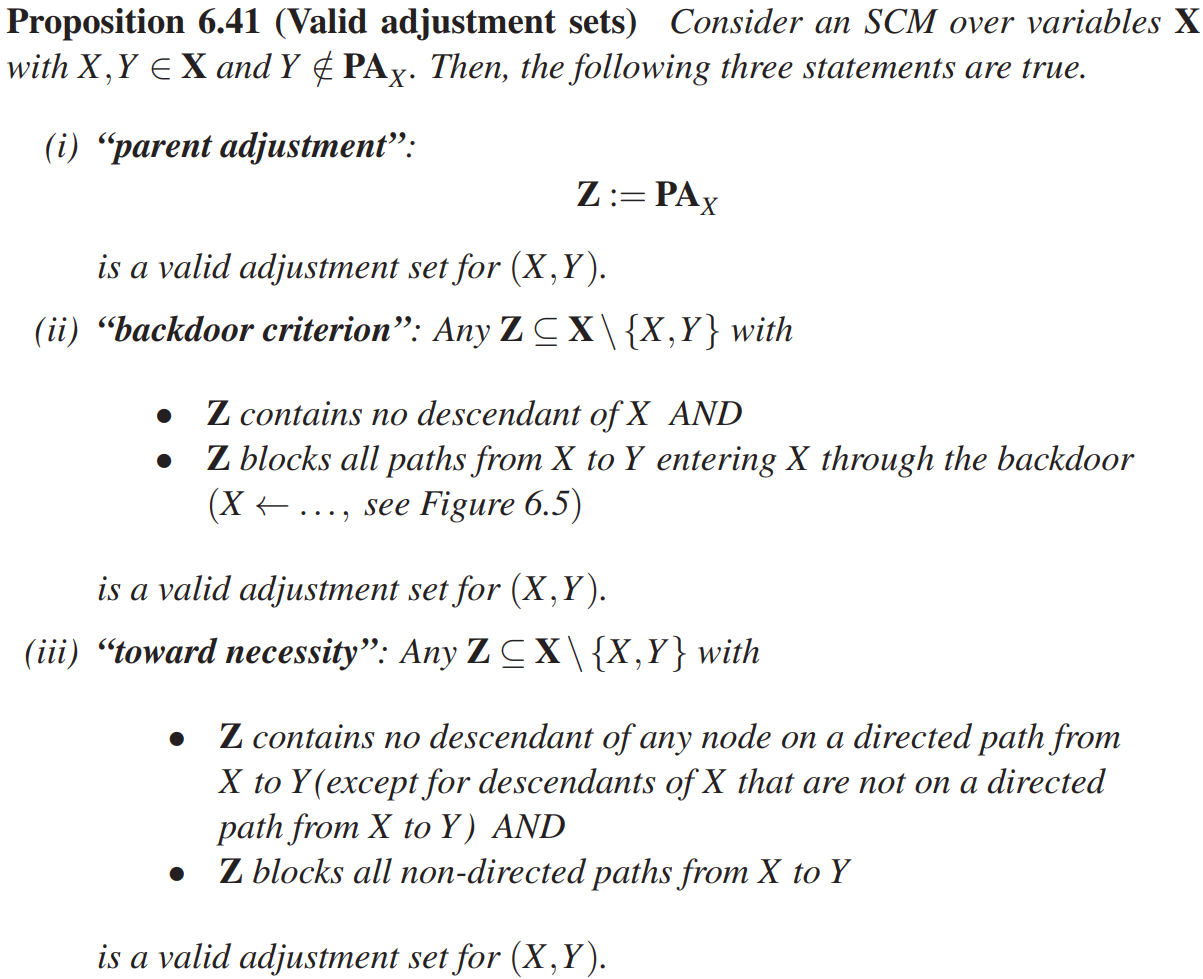
\includegraphics[scale=0.6]{fig17.png}}
\end{frame}

\begin{frame}
    \frametitle{Backdoor criterion}
    \centering{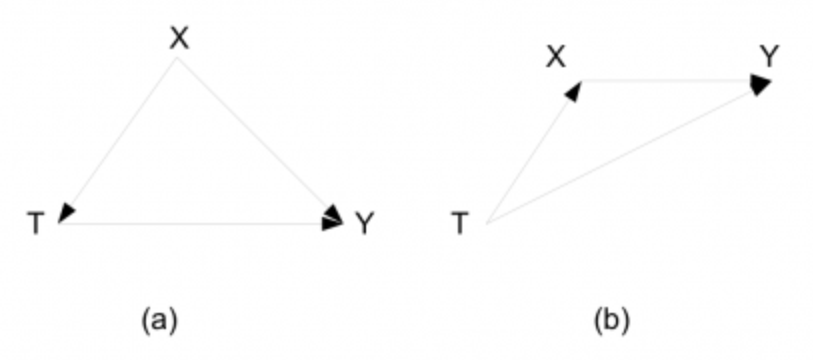
\includegraphics[scale=0.6]{fig30.png}}
    \begin{figure}[htbp]
        \centering
        \begin{minipage}[t]{0.48\textwidth}
        \centering
        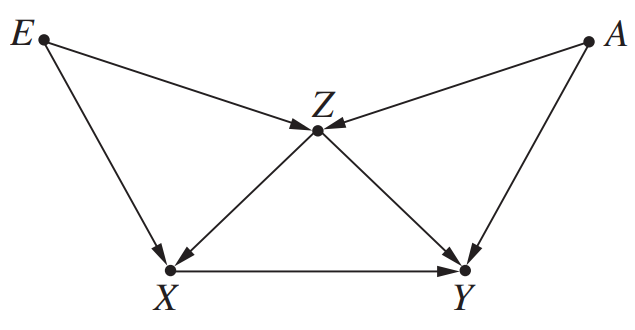
\includegraphics[scale=0.6]{fig32.png}
        \end{minipage}
        \begin{minipage}[t]{0.48\textwidth}
        \centering
        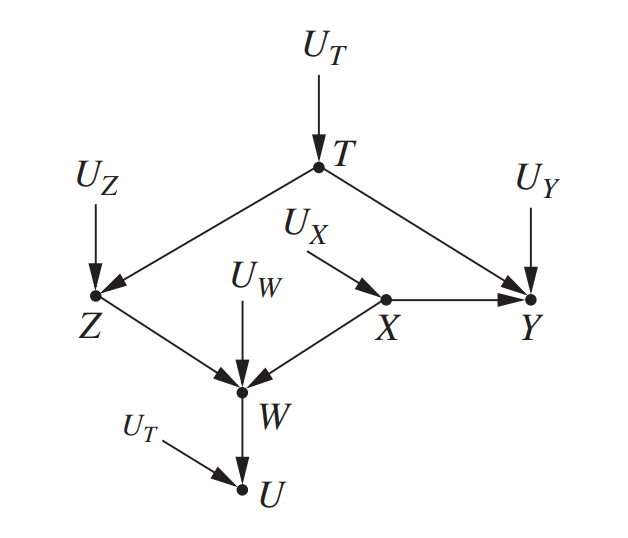
\includegraphics[scale=0.6]{fig31.png}
        \end{minipage}
    \end{figure}
\end{frame}

\begin{frame}
    \frametitle{Valid adjustment sets}
    \begin{flushleft}
        Suppose the valid adjustment set $Z$ is obtained via the backdoor criterion. We can then add any node $Z_0$ to 
        $Z$ that satisfies $Z_0\Vbar Y|X, Z$ because then
    \end{flushleft}
    \centering{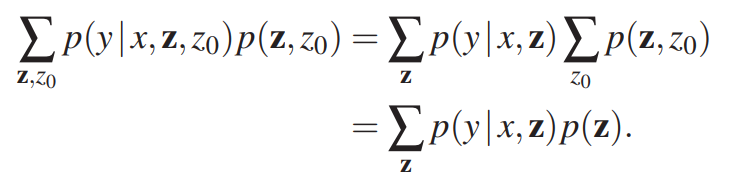
\includegraphics[scale=0.6]{fig29.png}}
    \begin{flushleft}
        In fact, Proposition (iii) characterizes all valid adjustment sets. 
    \end{flushleft}
\end{frame}

\begin{frame}
    \frametitle{Example}
    \centering{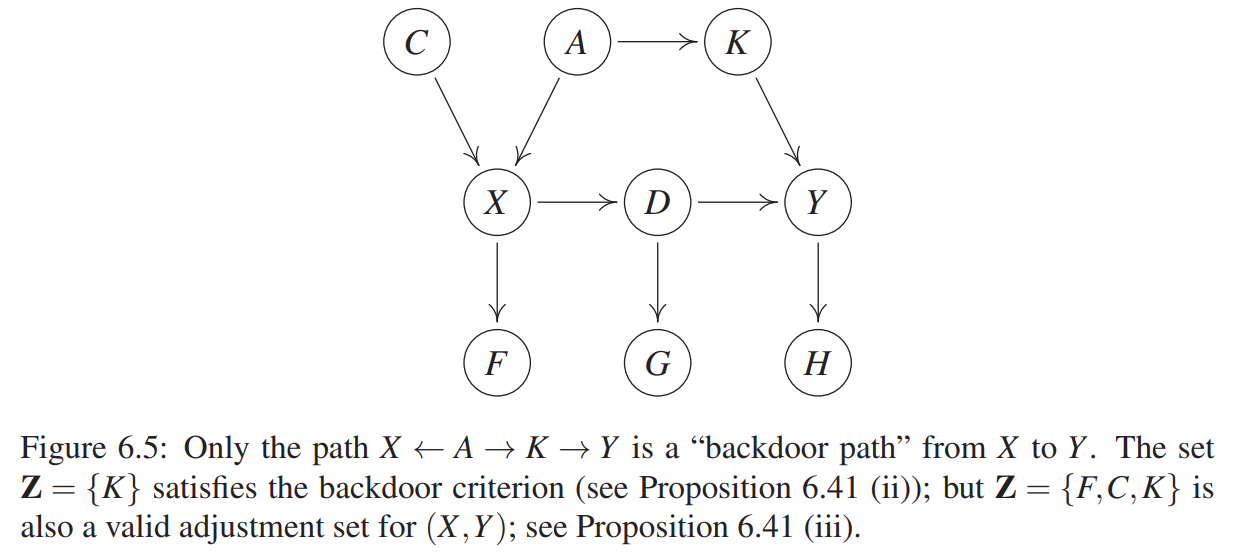
\includegraphics[scale=0.6]{fig18.png}}
\end{frame}



% \begin{frame}
    %\frametitle{Propensity score matching}
    %是causal里非常重要的方法!实在不行就放在第九章吧
%\end{frame}

\section{Do-Calculus}

\begin{frame}
    \frametitle{Contents}
    \tableofcontents[currentsection]
\end{frame}

\begin{frame}
    \frametitle{Front-door adjustment}
    \centering{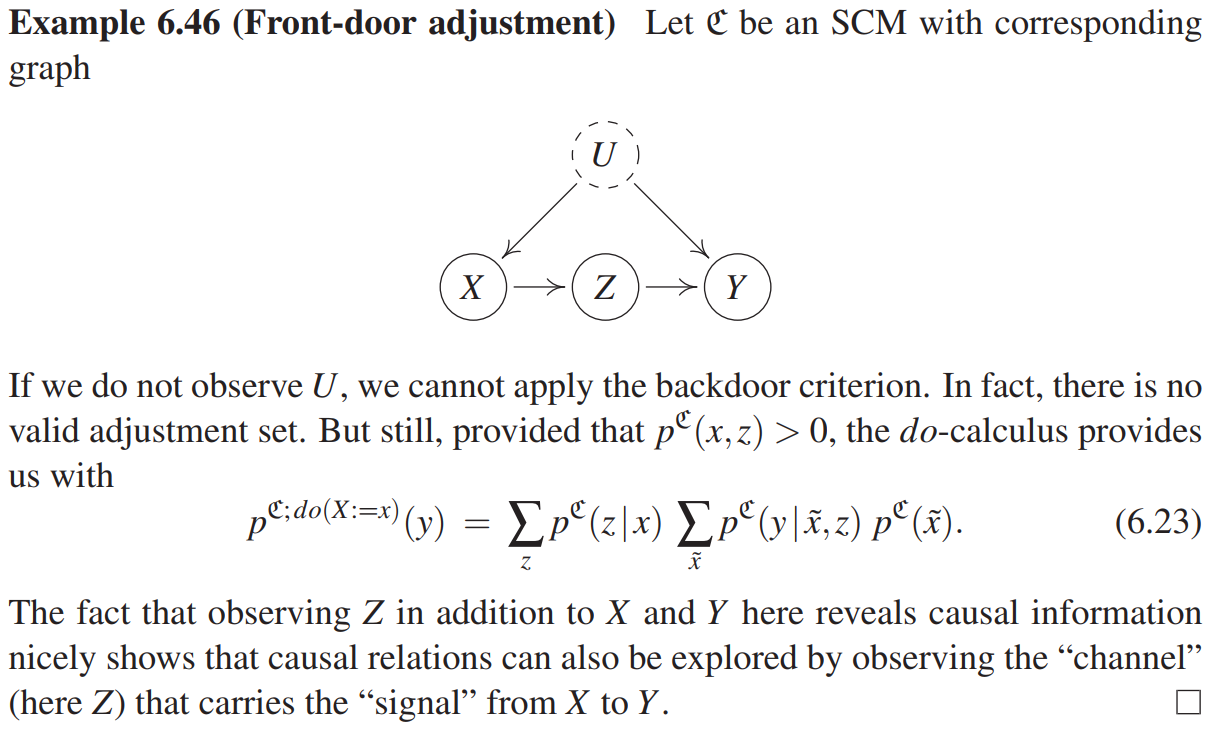
\includegraphics[scale=0.6]{fig21.png}}
\end{frame}

\begin{frame}
    \frametitle{Front-door adjustment}
    \centering{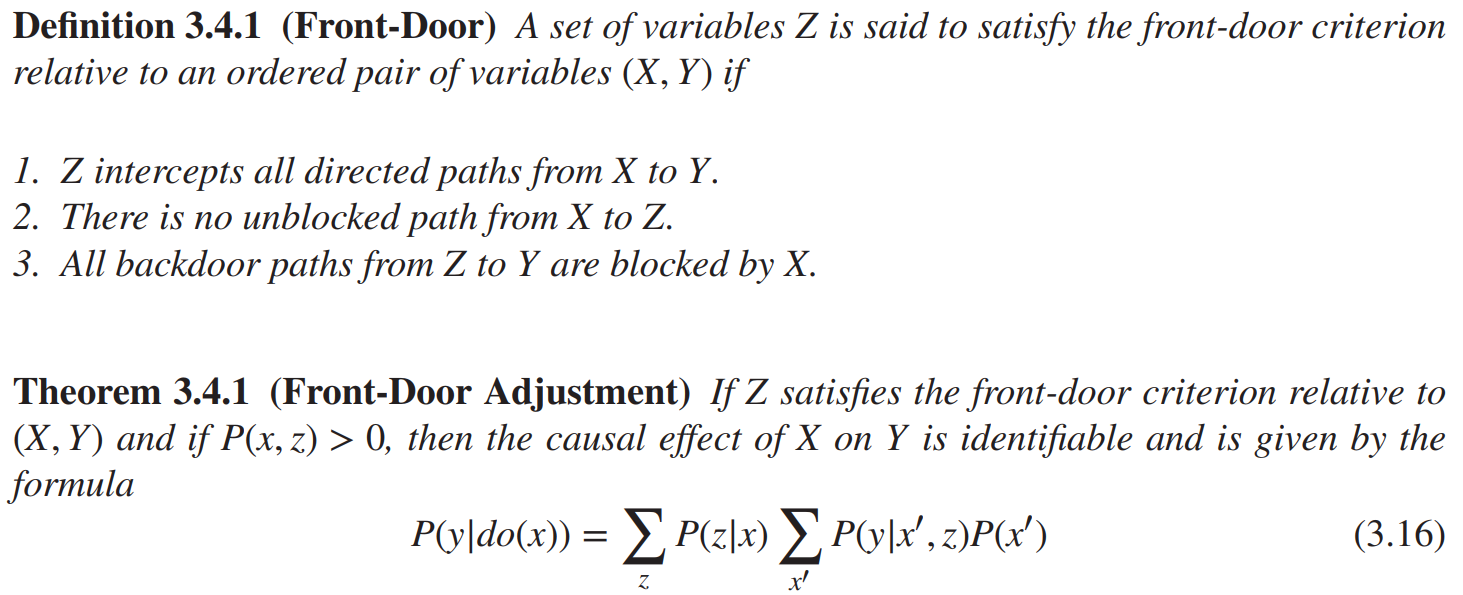
\includegraphics[scale=0.55]{fig33.png}}
\end{frame}

\begin{frame}
    \frametitle{Three rules}
    \begin{flushleft}
        Given a graph $\mathcal{G}$ and disjoint subsets $X$, $Y$, $Z$ and $W$, we have
    \end{flushleft}
    \centering{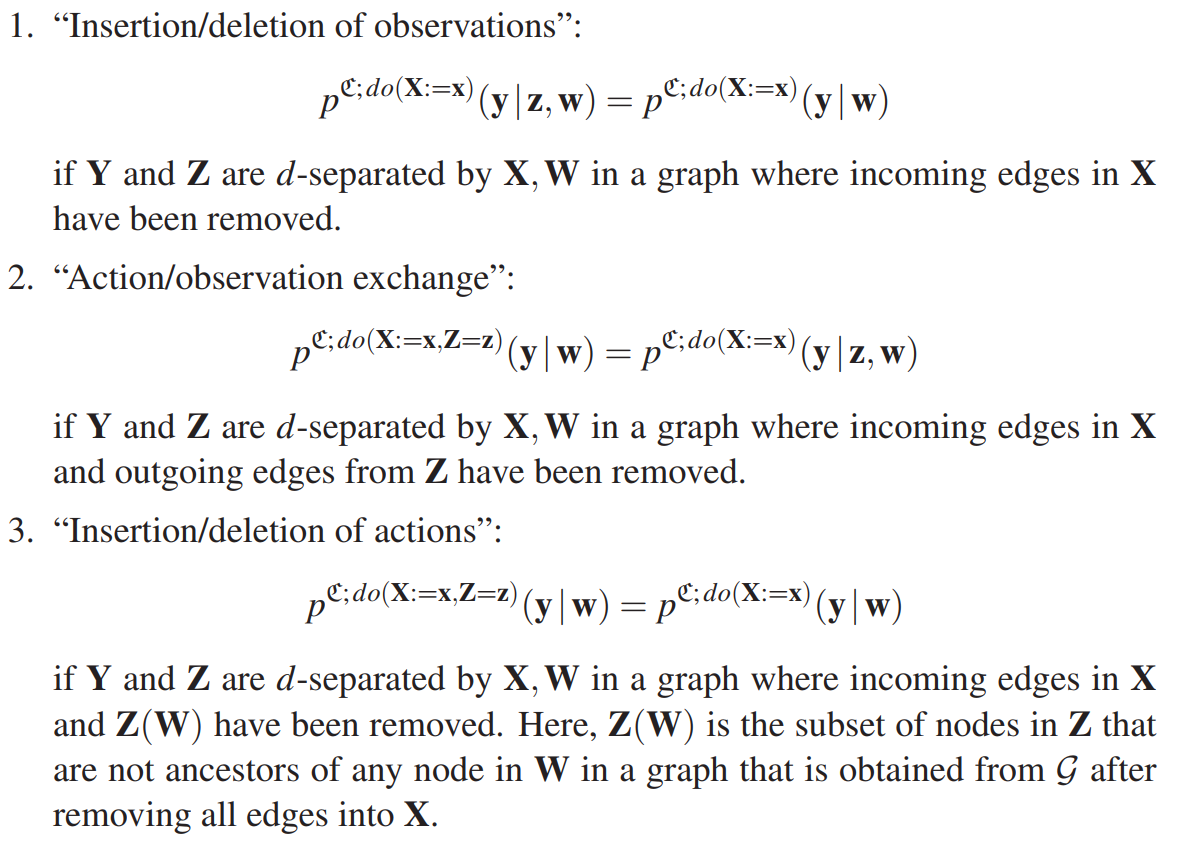
\includegraphics[scale=0.6]{fig19.png}}
\end{frame}

\begin{frame}
    \frametitle{Do-calculus}
    \begin{flushleft}
        We call an intervention distribution $p^{\mathfrak{C};do(X:=x)}(y)$ \textbf{identifiable} if it can be
        computed from the observational distribution and the graph structure. If there is a
        valid adjustment set for $(X;Y)$, $p^{\mathfrak{C};do(X:=x)}(y)$ is certainly identifiable.
    \end{flushleft}
    \centering{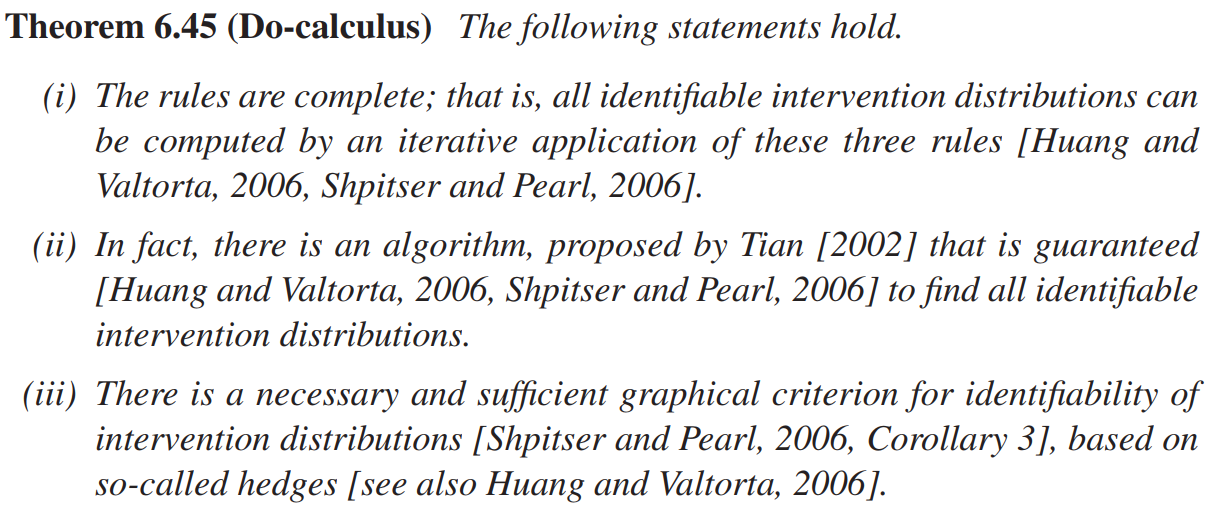
\includegraphics[scale=0.6]{fig20.png}}
\end{frame}

\section{Potential Outcomes}

\begin{frame}
    \frametitle{Contents}
    \tableofcontents[currentsection]
\end{frame}

\begin{frame}
    \frametitle{Example: the eye doctor}
    \begin{flushleft}
        For each unit $u$ we can observe either $B_u(t=1)$ or $B_u(t=0)$ and never both of them at the same time. They are
        called \textbf{potential outcomes}.
    \end{flushleft}
    \centering{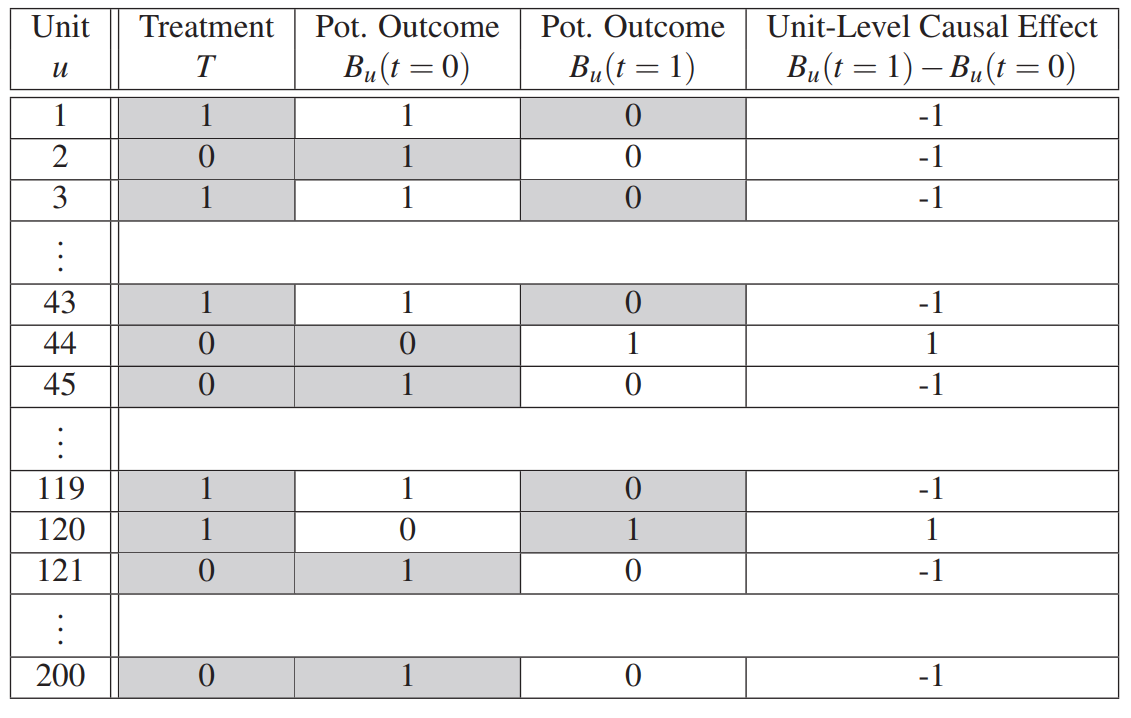
\includegraphics[scale=0.6]{fig23.png}}
\end{frame}

\begin{frame}
    \frametitle{Example: the eye doctor}
    The unit-level causal effect is
    \begin{align*}
        B_u(t=1) - B_u(t=0)
    \end{align*}
    The average causal effect is
    \begin{align*}
        CE = \frac{1}{n}\sum_{u=1}^n B_u(t=1) - B_u(t=0)
    \end{align*}
    Assume that in a completely randomized experiment, units $u\in U_0$ received treatment $T=0$ and 
    units $u\in U_1$ treatment $T = 1$, then
    \begin{align*}
        \widehat{CE}=\frac{1}{\# U_1}\sum_{u\in U_1}B_u(t=1) - \frac{1}{\# U_0}\sum_{u\in U_0}B_u(t=0)
    \end{align*}
    is an unbiased estimator. However, this solution is not reasonable due to the existence of
    \textbf{confounders}.
\end{frame}

\begin{frame}
    \frametitle{Potential outcome framework}
    \begin{flushleft}
        The core problem is: how to estimate the average causal effect $ACE=E(Y_i(1) - Y_i(0))$. \\
        If $Z\Vbar (Y(0),Y(1))$, it can be estimated as
    \end{flushleft}
    \centering{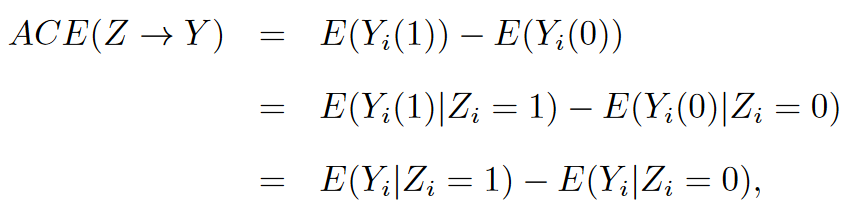
\includegraphics[scale=0.6]{fig25.png}}
    \begin{flushleft}
        However, $Z\Vbar (Y(0),Y(1))$ is violated due to the confounders. 
    \end{flushleft}
\end{frame}

\begin{frame}
    \frametitle{Assumptions}
    \begin{itemize}
        \item[$\bullet$] \textbf{Stable Unit Treatment Value Assumption(SUTVA)}: The potential outcomes for any unit do not 
        vary with the treatment assigned to other units, and, for each unit, there are no different forms or versions of each
        treatment level, which lead to different potential outcomes. \\
        \item[$\bullet$] \textbf{Ignorability}: Given the background variable $X$, treatment assignment $Z$ is independent of
        the potential outcomes. \\
    \end{itemize}
    \begin{flushleft}
        Under these assumptions, the average causal effect can be written as
    \end{flushleft}
    \centering{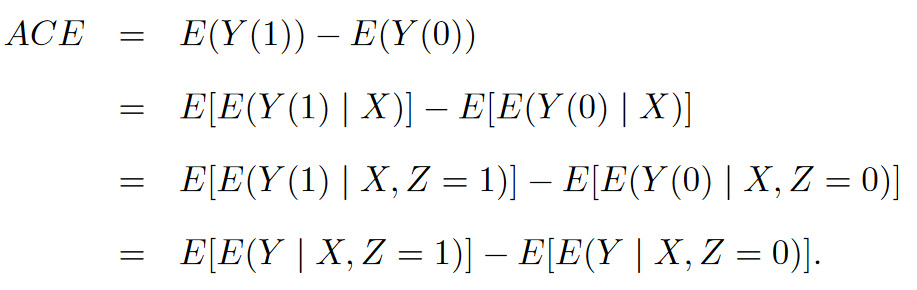
\includegraphics[scale=0.6]{fig24.png}}
\end{frame}

\begin{frame}
    \frametitle{Relation between Potential Outcomes and SCMs}
    \begin{flushleft}
        In SCMs, we can represent potential outcomes using the language of counterfactuals. 
    \end{flushleft}
    \centering{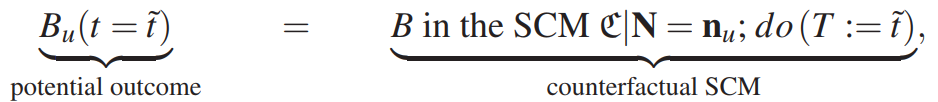
\includegraphics[scale=0.6]{fig22.png}}
    \begin{flushleft}
        The two representations are equivalent. Any theorem that holds for counterfactual SCMs holds
        in the world of potential outcomes and vice versa. 
    \end{flushleft}
\end{frame}





% \section{Equivalence and Falsifiability of Causal Models}

% \begin{frame}
%     \frametitle{Contents}
%     \tableofcontents[currentsection]
% \end{frame}

% \begin{frame}
%     \frametitle{Equivalence of causal models}
%     \centering{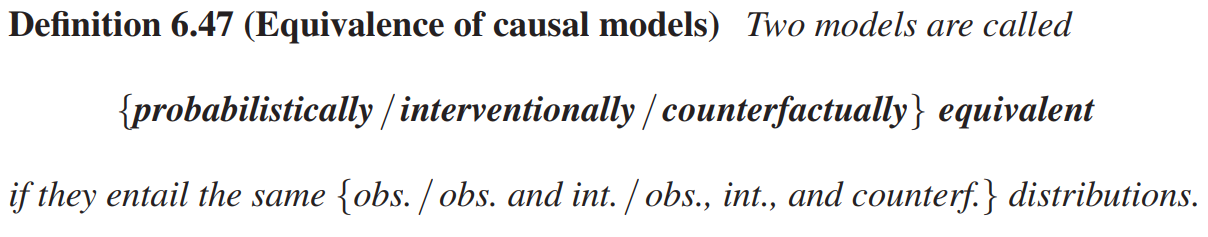
\includegraphics[scale=0.6]{fig1.png}}
% \end{frame}

% \begin{frame}
%     \frametitle{Interventional equivalence}
%     \centering{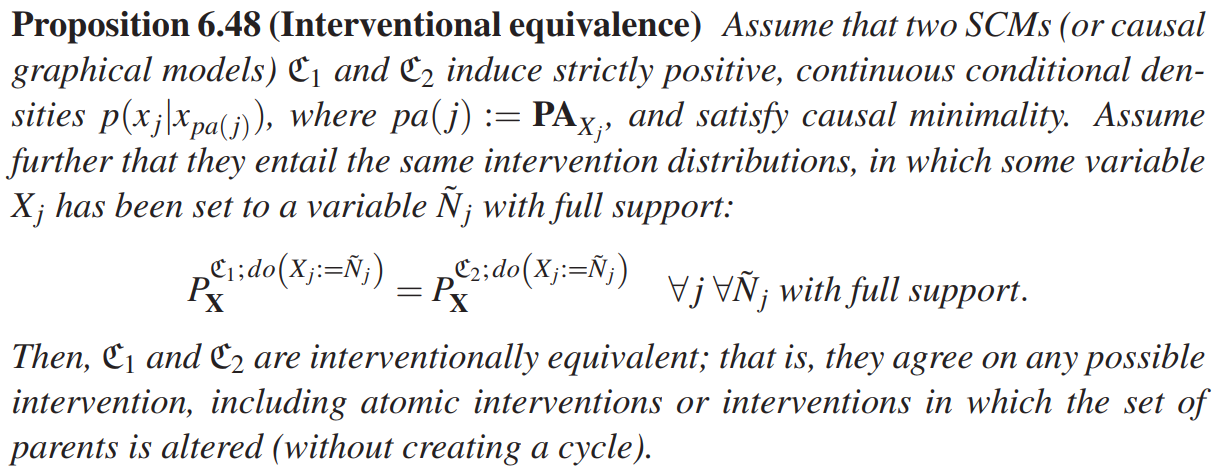
\includegraphics[scale=0.6]{fig2.png}}
% \end{frame}

% \begin{frame}
%     \frametitle{Counterfactual equivalence}
%     \centering{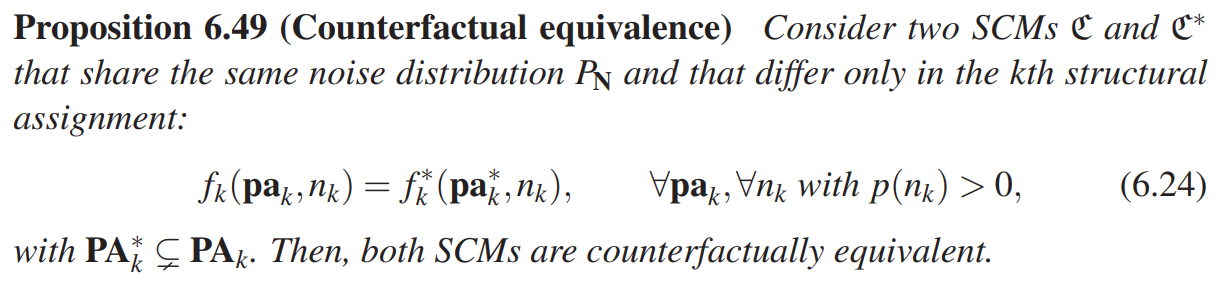
\includegraphics[scale=0.6]{fig3.png}}
% \end{frame}



% \section{Generalized Structural Causal Models Relating Single Objects}

% \begin{frame}
%     \frametitle{Contents}
%     \tableofcontents[currentsection]
% \end{frame}

% \section{Algorithmic Independence of Conditionals}

% \begin{frame}
%     \frametitle{Contents}
%     \tableofcontents[currentsection]
% \end{frame}

\begin{frame}
    \frametitle{Reference} 
    Pearl J, Glymour M, Jewell N P. Causal inference in statistics: A primer[M]. John Wiley \& Sons, 2016. \\
    Yao L, Chu Z, Li S, et al. A Survey on Causal Inference[J]. ACM Transactions on
    Knowledge Discovery from Data (TKDD), 2021, 15(5): 1-46. \\
    https://www.math.pku.edu.cn/teachers/yaoy/math112230/ \\
\end{frame}


\end{document}
